\documentclass[10pt,a4paper]{article}
\usepackage[utf8]{inputenc}
\usepackage[T1]{fontenc}
\usepackage{amsmath}
\usepackage{amssymb}
\usepackage{graphicx}
\usepackage{nicematrix}
\usepackage[left=2.00cm, right=2.00cm, top=2.00cm, bottom=2.00cm]{geometry}
\usepackage{float}
\usepackage{caption}
\usepackage{subcaption}
\usepackage{multirow}
\usepackage{diagbox}
\usepackage{color}
\usepackage[
	colorlinks=true,
	linkcolor=blue,
	filecolor=blue,      
	urlcolor=cyan,
	citecolor=cyan,    
]{hyperref}
\usepackage{algorithm}
\usepackage{algpseudocode}

\title{\textbf{CIE6107 - Robotics and Intelligent Systems \\Assignment 1}}
\author{Zixing JIANG}
\begin{document}
	
\begin{flushleft}
	CSC3180: Fundamentals of Artificial Intelligence, Spring 2023\\
	Project Report, Group 10\\
	\today
\end{flushleft}
	
\begin{flushright}\vspace{-18mm}
	
\includegraphics[height=1.7cm]{figure/logo.png}
\end{flushright}
	
\begin{center}\vspace{0.5cm}
	\textbf{\Large Adaptive Dynamic Stabilization of a Self-Balancing Scooter Using Epsilon-Greedy Q-learning}\\~\\
	\large Hongyi Yang, Muhan Lin, Xuanyang Xu, Zixing Jiang
\end{center}
{\noindent}\rule{\linewidth}{0.1mm}

\section{Introduction}
The self-balancing scooter (Figure \ref{fig:scooter}) is a common urban commuter tool. One of the most critical features in self-balancing scooter is dynamic stabilization,  which allows the scooter to maintain its balance while in motion. Without this feature, it would be very difficult for riders to stay upright and control the scooter, and even cause safety accidents in severe cases. In order to achieve dynamic stabilization, the traditional automatic control methods, including Proportional-Integral-Derivative (PID) control and Model Predictive Control (MPC), model the self-balancing scooter as a cart-pole system (Figure \ref{fig:cart-pole}) and designs the controller by deriving its system dynamics. However, the dynamics-based control is sensitive to the rider's weight and center of mass (CoM). For riders of different weights and CoMs, the performance of stabilization varies. In this project, we aim to utilize the learning ability of artificial intelligence to design a dynamic stabilizer that adapts to different rider weights and CoMs.

\begin{figure}[H]
	\centering
	\begin{subfigure}[b]{0.3\textwidth}
		\centering
		
\includegraphics[width=0.5\textwidth]{figure/scooter}
		\caption{Man on a self-balancing scooter}
		\label{fig:scooter}
	\end{subfigure}
	\hfill
	\begin{subfigure}[b]{0.3\textwidth}
		\centering
		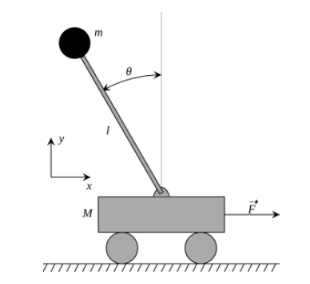
\includegraphics[width=0.85\textwidth]{figure/cart-pole}
		\caption{Cart-pole system dynamics}
		\label{fig:cart-pole}
	\end{subfigure}
	\hfill
	\begin{subfigure}[b]{0.3\textwidth}
		\centering
		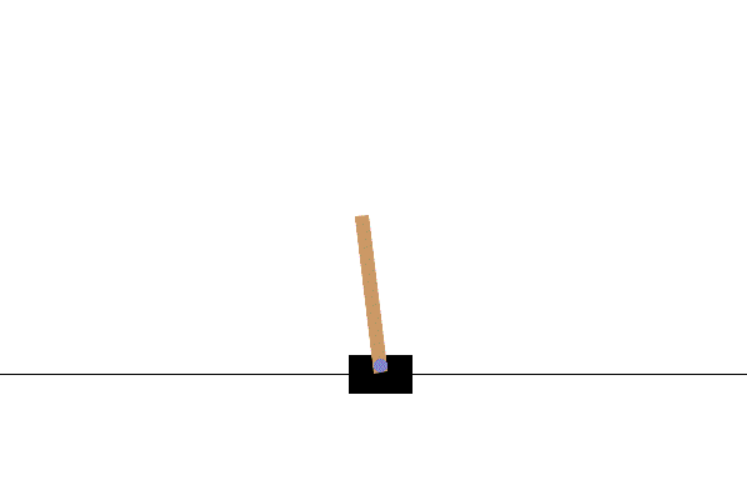
\includegraphics[width=\textwidth]{figure/open-ai}
		\caption{OpenAI Cart Pole Environment}
		\label{fig:openai}
	\end{subfigure}
	\caption{Illustrations of (a) the self-balancing scooter, (b) the cart-pole system dynamics, and (c) the OpenAI Cart Pole environment.}
	\label{fig:three graphs}
\end{figure}

\section{Problem Statement}
In this project, we model the scooter as the cart-pole system (Figure \ref{fig:cart-pole}). The wheel of scooter is the cart the rider-scooter mass is the pole. Then the adaptive stabilization problem can be formulated as follows: control the inclination ($\theta$) of a pole with \textcolor{red}{varying mass and CoM} within a certain range by controlling the movement ($x$) of the cart (leftward or rightward).  We intend to apply reinforcement learning (RL) to solve this problem. Namely, given the observation of the environment ($\theta, \dot{\theta}, x, \dot{x}$), we want our agent (cart) to learn a policy (move leftward or move rightward) to stable the varying pole through trail and reward. We plan to implement our RL algorithm based on the \href{https://gymnasium.farama.org/environments/classic_control/cart_pole/}{OpenAI Gym environment for cart-pole} (Figure \ref{fig:openai}). 

\section{Epsilon-Greedy Q-Learning}
In this project, we built our dynamic stabilization controller with Epsilon-Greedy Q-Learning, which is a well-developed reinforcement learning algorithm that balances exploration and exploitation in sequential decision-making problems. In this section, we will introduce the Epsilon-Greedy Q-Learning algorithm in detail and explain how we link this algorithm to the dynamic balancing problem we aim to solve. 

\subsection{Q-Learning}
Q-Learning is a classic value-based reinforcement learning algorithm that allow an agent to learn from its own actions and rewards in an environment. Unlike some other model-based control and reinforcement learning methods, it does not require a model of the environment. This feature helps to solve the traditional model-based control method's dependence on the rider's center of gravity mentioned in previous sections. 

The goal of Q-Learning is to find an optimal policy that maximizes the expected value of the total reward over any sequence of actions. The main idea of Q-Learning is to use a table, called Q-Table, that stores the estimated value $Q(\boldsymbol{s}, \boldsymbol{a})$ (Q-Value) of each action $\boldsymbol{a}$ in each state $\boldsymbol{s}$, as shown in Table \ref{tab:q-table}. The Q-Value, which reflects the value of taking a certain action in a certain state, is defined as the expectation of overall received rewards after taking action $\boldsymbol{a}$ at state $\boldsymbol{s}$, as shown in \eqref{eq:q-value}. 
\begin{equation}
	Q(\boldsymbol{s}, \boldsymbol{a}) = \mathbb{E}\left(\sum_{t = 0}^{\infty} \gamma^{t}r(\boldsymbol{s}_{t}, \boldsymbol{a}_{t}) ~\left|~ \boldsymbol{s}_{0} = \boldsymbol{s}, \boldsymbol{a}_{0} = \boldsymbol{a}\right.\right)
	\label{eq:q-value}
\end{equation}
where $r(\boldsymbol{s}_{t}, \boldsymbol{a}_{t})$ is the reward received from the environment for state-action pair $(\boldsymbol{s}_{t}, \boldsymbol{a}_{t})$ and $\gamma$ is the discount factor. 

In Q-Learning, in order to obtain the most accurate estimate of the Q-Value,  the Bellman Equation is applied to update $Q(\boldsymbol{s}, \boldsymbol{a})$ in every iteration that state-action pair $(\boldsymbol{s}, \boldsymbol{a})$ is chosen, as shown in \eqref{eq:bellman}
\begin{equation}
	\text{New~} Q(\boldsymbol{s}, \boldsymbol{a}) \leftarrow (1-\lambda)\text{Current~} Q(\boldsymbol{s}, \boldsymbol{a}) + \lambda \left[ r(\boldsymbol{s}, \boldsymbol{a}) + \gamma \max_{\boldsymbol{a'}}Q(\boldsymbol{s'}, \boldsymbol{a'})\right]
	\label{eq:bellman}
\end{equation}
where $r(\boldsymbol{s}, \boldsymbol{a})$ is the reward received in this iteration, $\boldsymbol{s'}$ is the transient state after taking $\boldsymbol{a}$ at $\boldsymbol{s}$, $\boldsymbol{a'}$ is the legal action at $\boldsymbol{s'}$, $\gamma$ is the discount factor, and $\lambda$ is the learning rate. 

In the Q-Learning process, the agent updates the Q-Table as it explores the environment and receives feedback. The agent chooses the action $\boldsymbol{a}^{*}(\boldsymbol{s})$ that has the highest value in the current state $\boldsymbol{s}$, according to the Q-Table, as shown in \eqref{eq:action-selection}.  
\begin{equation}
	\boldsymbol{a}^{*}(\boldsymbol{s}) = \arg\max_{\boldsymbol{a}}Q(\boldsymbol{s}, \boldsymbol{a})
	\label{eq:action-selection}
\end{equation}
This way, the agent learns to act optimally over time.

In our scenario, the state vector $\boldsymbol{s}$ of the cart-pole system is continuous. In order to prevent infinitely many state-action pairs, we discretized the system's state space by intervals. The length of each interval is fine-tuned to ensure the effectiveness of learning. Plus, since the Q-Table is keeping updating during the algorithm runtime, it is adaptive to dynamic environment parameters. Therefore the stabilization controller built with Q-Learning is capable of adapting to varying rider weights and CoMs.

\begin{table}
\centering
\begin{tabular}{|c|c|c|c|c|}
\hline
\diagbox{States}{Actions}& $\boldsymbol{a}_{0}$ & $\boldsymbol{a}_{1}$ & $\boldsymbol{a}_{2}$ & \dots \\
\hline
$\boldsymbol{s}_{0}$ & $Q(\boldsymbol{s}_{0}, \boldsymbol{a}_{0})$ & $Q(\boldsymbol{s}_{0}, \boldsymbol{a}_{1})$ & $Q(\boldsymbol{s}_{0}, \boldsymbol{a}_{2})$ & \dots \\
\hline
$\boldsymbol{s}_{1}$ & $Q(\boldsymbol{s}_{1}, \boldsymbol{a}_{0})$ & $Q(\boldsymbol{s}_{1}, \boldsymbol{a}_{1})$ & $Q(\boldsymbol{s}_{1}, \boldsymbol{a}_{2})$ & \dots \\
\hline
$\boldsymbol{s}_{2}$ &$Q(\boldsymbol{s}_{2}, \boldsymbol{a}_{0})$ & $Q(\boldsymbol{s}_{2}, \boldsymbol{a}_{1})$ & $Q(\boldsymbol{s}_{2}, \boldsymbol{a}_{2})$ & \dots \\
\hline
$\boldsymbol{s}_{3}$ & $Q(\boldsymbol{s}_{3}, \boldsymbol{a}_{0})$ & $Q(\boldsymbol{s}_{3}, \boldsymbol{a}_{1})$ & $Q(\boldsymbol{s}_{3}, \boldsymbol{a}_{2})$ & \dots \\
\hline
\dots & \dots & \dots & \dots & \dots \\
\hline
\end{tabular}
\caption{An example of Q-Table. $Q(\boldsymbol{s}_{i}, \boldsymbol{a}_{j})$ denotes the Q-Value of a state-action pair ($\boldsymbol{s}_{i}, \boldsymbol{a}_{j}$). The higher $Q(\boldsymbol{s}_{i}, \boldsymbol{a}_{j})$ is, the more worthy to take action $\boldsymbol{a}_{j}$ at state $\boldsymbol{s}_{i}$. } 
\label{tab:q-table}
\end{table}

\subsection{Epsilon-Greedy Action Selection}
In order to learn an optimal Q-table, we want our algorithm to explore all possible state-action pairs. Thus, in addition to the action selection criterion \eqref{eq:action-selection},  an epsilon-greedy policy is applied. Given an epsilon-greedy factor $0 \le \varepsilon \le 1$, in each iteration, there is a probability of $\varepsilon$ that the agent takes random actions to explore new possible state-action pairs, and there is a probability of $1 - \varepsilon$ that the agent exploits investigated state-action pairs via the Q-Table. The overall logic flow of the Epsilon-Greedy Q-Learning is shown in algorithm \ref{alg:egql}. 

\begin{algorithm}
\caption{Epsilon-Greedy Q-Learning}\label{alg:egql}
\begin{algorithmic}
\Require observation of state $\boldsymbol{s}$, epsilon-greedy factor $\varepsilon \in [0,1]$
\While{learning not terminate}
\State Generate a random number $i \in [0,1]$
\If{$i \le \varepsilon$}
\State Take random action $\boldsymbol{a}$
\Else
\State Select action $\boldsymbol{a}$ according to the Q-Table \Comment{Equation \eqref{eq:action-selection}}
\EndIf
\State Update Q-Table entry for $(\boldsymbol{s}, \boldsymbol{a})$ according to the received reward $r(\boldsymbol{s}, \boldsymbol{a})$ \Comment{Equation \eqref{eq:bellman}}
\EndWhile

\end{algorithmic}
\end{algorithm}

\end{document}